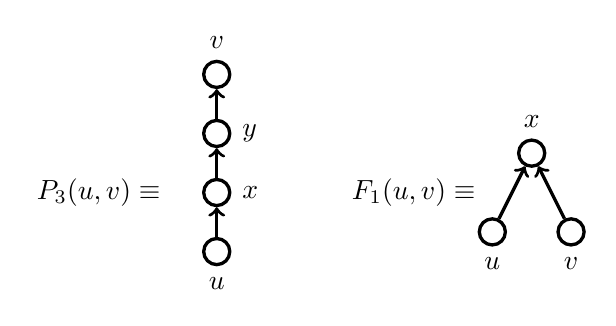
\begin{tikzpicture}[
    scale=0.5,
    line width=1.2pt
]

    \node at (-7,-3) {\(P_3(u,v)\equiv\)};
    
    \node[circle, draw=black, fill=white, label=below:{\(u\)}]
            (p0) at (-4,-4.5) {};

    \node[circle, draw=black, fill=white, label=right:{\(x\)}]
            (p1) at (-4,-3) {};
    \node[circle, draw=black, fill=white, label=right:{\(y\)}]
            (p2) at (-4,-1.5) {};

    \node[circle, draw=black, fill=white,
    label=above:{\(v\)}]
        (p3) at (-4,0) {};
    

    \draw[->] (p0) -- (p1);
    \draw[->] (p1) -- (p2);
    \draw[->] (p2) -- (p3);

\onslide<2>{
    \node at (1,-3) {\(F_1(u,v)\equiv\)};
    
    \node[circle, draw=black, fill=white, label=below:{\(u\)}]
            (p0) at (3,-4) {};

    \node[circle, draw=black, fill=white, label=below:{\(v\)}]
            (p1) at (5,-4) {};

    \node[circle, draw=black, fill=white, label=above:{\(x\)}]
        (p2) at (4,-2) {};
    

    \draw[->] (p0) -- (p2);
    \draw[->] (p1) -- (p2);
}

\end{tikzpicture}